\documentclass[sigconf, authordraft, capitalise]{acmart}

\usepackage{tcolorbox}
\usepackage{listings}
\usepackage{tikz}
\usepackage{flafter}
\usepackage{booktabs}

\usetikzlibrary{calc}
\usetikzlibrary{graphs}
\usetikzlibrary{shapes}
\usetikzlibrary{positioning}
\usetikzlibrary{arrows.meta}

\lstloadlanguages{PHP}
\lstset{language=PHP,basicstyle=\footnotesize\ttfamily}


% \title{(Mis)using unit testing to semi-automatically grade SQL schemas}
\title{Semi-automated grading of SQL schemas \\ by (mis)use of database unit testing}
\author{Nigel Stanger}
\orcid{orcid.org/0000-0003-3450-7443}
\affiliation{
    \institution{University of Otago}
    \department{Department of Information Science}
    \city{Dunedin}
    \country{New Zealand}
}
\email{nigel.stanger@otago.ac.nz}

\begin{document}

\begin{abstract}
    abstract
\end{abstract}

\maketitle


\section{Introduction}

Any introductory database course needs to cover several core concepts, such as what is a database, what is a logical data model, and how to create and interact with a database. Typically such courses focus on the Relational Model and its embodiment in SQL database management systems (DBMSs). This is partly because the Relational Model provides a sound theoretical framework for discussing key database concepts \cite{Date.C-2009a-SQL-and-Relational}, and partly because SQL DBMSs are still widely used. The shadow of SQL is so strong that even non-relational systems have adopted some form of SQL-like language in order to leverage existing knowledge (e.g., OQL \cite{Cattell.R-2000a-ODMG3}, HiveQL \cite{Apache-2017a-Hive}, and CQL \cite{Apache-2017a-CQL}).

Courses that teach SQL usually include one or more assessments that test students' ability to create a database using SQL data definition (DDL) statements, and to interact with the database using SQL data manipulation (DML) statements. Manually grading the code submitted for such assessments can be a slow, tedious, and potentially error-prone process. Automated or semi-automated grading has been shown to improve turnaround time and consistency, and is generally received positively by students \cite{Douce.C-2005a-Automatic,Russell.G-2004a-Improving,Dekeyser.S-2007a-Computer,Prior.J-2004a-Backwash}. If the grading can be done in real time, the grading tool can even become part of a larger, interactive SQL learning environment (e.g.,  \cite{Kenny.C-2005a-Automated,Kleiner.C-2013a-Automated,Mitrovic.A-1998a-Learning,Russell.G-2004a-Improving,Sadiq.S-2004a-SQLator}).

While there have been many prior efforts to automatically grade SQL DML (see \cref{sec-literature}), there appear to be no similar systems designed to automatically grade SQL \emph{DDL}. There are generally two main aspects that need to be considered when grading an SQL schema implementation. First, is the DDL code (i.e., \texttt{CREATE} statements) syntactically correct? This is already dealt with quite effectively by the syntax checkers built into every SQL DBMS (although it is fair to say that the errors produced by such checkers can sometimes be obscure and unhelpful). Any student who submits syntactically invalid code cannot expect to score well. A related aspect is code style (e.g., naming, formatting, indentation), but we do not consider this here.
    
Second, does the schema meet the requirements of the problem being solved? A database schema is normally designed and implemented within the context of a specific set of requirements, so verifying that the implemented SQL schema fulfils these requirements is an effective way to grade the implementation, and also provides a useful framework for providing feedback to students. The requirements for a database schema can usually be loosely divided into \emph{structure} (e.g., tables, columns, data types), \emph{integrity} (e.g., keys, constraints), and \emph{behaviour} (e.g., sequences, triggers).

In this paper we describe a system that semi-automates the grading of SQL schema implementations. The system takes as input a machine-readable specification of the assessment requirements and a live instance of a submitted student schema, and checks whether the schema conforms to the requirements. Rather than attempt to parse and check the \texttt{CREATE TABLE} statements directly, the system instead issues queries on the schema's metadata (catalog), and compare the results of these queries against the machine-readable specification. The process effectively becomes one of unit testing the schema using the specification as a framework. We use the PHPunit database unit testing framework to carry out this process, albeit in a somewhat unorthodox way (see \cref{sec-design}).

The remainder of the paper is structured as follows. In the next section we discuss related work and identify gaps, while \cref{sec-motivation} discusses the motivation for our approach. \Cref{sec-design} discusses the design of our system, and \cref{sec-evaluation} evaluates its effectiveness. We conclude in \cref{sec-conclusion}.


\section{Related work}
\label{sec-literature}

There have been many prior efforts to build learning systems for SQL. However, these have focused almost exclusively on SQL queries using the \texttt{SELECT} statement (i.e., DML) rather than schema definitions (DDL). This is unsurprising given the relative complexity of the \texttt{SELECT} statement compared to most other SQL statements.

\citeauthor{Dietrich.S-1993a-An-educational}'s \emph{RDBI} \cite{Dietrich.S-1993a-An-educational} was a Prolog-based interpreter for relational algebra, tuple and domain relational calculus, and SQL. It focused primarily on queries, and used its own non-SQL data definition language. RDBI did not provide feedback on students' attempts beyond basic syntax checking and displaying query results. 

\citeauthor{Kearns.R-1997a-A-teaching}'s \emph{esql} \cite{Kearns.R-1997a-A-teaching} supported students in learning the fundamental concepts underlying SQL. It could parse and execute \texttt{CREATE}, \texttt{DROP}, \texttt{ALTER}, \texttt{DELETE}, \texttt{INSERT}, and \texttt{SELECT} statements, but all of these except \texttt{SELECT} were simply passed through to the DBMS. The system enabled students to better understand the steps in the execution of a query by visualizing the intermediate tables generated by each step of the query. It did not provide feedback on students' attempts beyond basic syntax checking and displaying query results.

\citeauthor{Mitrovic.A-1998a-Learning}'s \emph{SQL-Tutor} \cite{Mitrovic.A-1998a-Learning} was an intelligent teaching system  that provided students with a guided discovery learning environment for SQL queries. It supported only the \texttt{SELECT} statement, and used constraint-based modeling \cite{Ohlsson.S-1992a-Constraint-based,Ohlsson.S-2016a-Constraint-based} to provide feedback to students on both syntactic and semantic SQL errors.

\citeauthor{Sadiq.S-2004a-SQLator} \emph{SQLator} \cite{Sadiq.S-2004a-SQLator} was a web-based interactive tool for learning SQL. Students were presented with a series of questions in English, and had to write SQL \texttt{SELECT} statements to answer these questions. SQLator used an ``equivalence engine'' to determine whether an SQL query fulfilled the requirements of the original English question. SQLator supported only the \texttt{SELECT} statement, and provided only basic feedback (correct or incorrect) to students. SQLator was able to automatically mark about a third of submitted queries as correct, thus improving the speed of grading. 

\citeauthor{Prior.J-2004a-Backwash}'s \emph{AsseSQL} \cite{Prior.J-2004a-Backwash} was an online examination environment for evaluating students' ability to formulate SQL queries. Students would write and execute their queries, and the data set produced by their query would be compared against the correct data set. The answer would then be flagged as correct or incorrect as appropriate. AsseSQL supported only the \texttt{SELECT} statement.

\citeauthor{Russell.G-2004a-Improving}'s \emph{ActiveSQL}\footnote{\url{https://db.grussell.org/}} \cite{Russell.G-2004a-Improving,Russell.G-2005a-Online} was an online interactive learning environment for SQL that provided immediate feedback to students. ActiveSQL measured the accuracy of a query in a similar way to \citeauthor{Prior.J-2004a-Backwash}'s AsseSQL, but instead of a simple correct/incorrect answer, it computed an accuracy score based on the differences between the query output and the correct answer. It was also able to detect ``hard-coded'' queries that produced the desired result, but would fail if the data set changed \cite{Russell.G-2005a-Online}. ActiveSQL supported only the \texttt{SELECT} statement.

\citeauthor{Dekeyser.S-2007a-Computer}'s \emph{SQLify} \cite{Dekeyser.S-2007a-Computer} was another online SQL learning system that incorporated semantic feedback and automatic assessment. SQLify evaluated each query on an eight-level scale that covered query syntax, output schema, and query semantics. Instructors could use this information to award an overall grade. Again, SQLify supported only the \texttt{SELECT} statement.

\citeauthor{Brusilovsky.P-2010a-Learning}'s \emph{SQL Exploratorium} \cite{Brusilovsky.P-2010a-Learning} took an interesting approach to generating problems, using parameterised query templates to generate the questions given to students. Again, the SQL Exploratorium supported only the \texttt{SELECT} statement.

\citeauthor{Kleiner.C-2013a-Automated}'s \emph{aSQLg} \cite{Kleiner.C-2013a-Automated} was an automated assessment tool that provided feedback to students. This enabled students to improve their learning by making further submissions after incorporating this feedback. The aSQLg system checked queries for syntax, efficiency (cost), result correctness, and statement style. Again, aSQLg supported only the \texttt{SELECT} statement.

\citeauthor{Kenny.C-2005a-Automated} \cite{Kenny.C-2005a-Automated} described an SQL learning system similar to those already described, which also incorporated an assessment of a student's previous progress. This enabled a more personalized and adaptive approach to student learning, where feedback was tailored according to student progress. Again, this system supported only the \texttt{SELECT} statement.

\citeauthor{Bhangdiya.A-2015a-XDa-TA}'s \emph{XDa-TA}\footnote{\url{http://www.cse.iitb.ac.in/infolab/xdata/}} extended the idea of automated grading of SQL by adding the ability to generate data sets designed to catch common errors. These data sets were automatically derived from a set of correct SQL queries \cite{Bhangdiya.A-2015a-XDa-TA,Chandra.B-2015a-Data}. Later work \cite{Chandra.B-2016a-Partial} added support for awarding partial marks.

\citeauthor{Gong.A-2015a-CS-121-Automation}'s ``CS 121 Automation Tool'' \cite{Gong.A-2015a-CS-121-Automation} was a tool designed to semi-automate the grading of SQL assessments, again focusing on SQL DML statements. Interestingly, the system appears to be extensible and could thus potentially be modified to support grading of \texttt{CREATE TABLE} statements.

There is relatively little work on unit testing of databases. Most authors working in this area have focused on testing database \emph{applications} rather than the database itself (e.g., \cite{Binnig.C-2008a-Multi-RQP,Chays.D-2008a-Query-based,Marcozzi.M-2012a-Test,Haller.K-2010a-Test}). \citeauthor{Ambler.S-2006a-Database} discusses how to test the functionality of a database \cite{Ambler.S-2006a-Database}, while \citeauthor{Farre.C-2008a-SVTe} test the ``correctness'' of a schema \cite{Farre.C-2008a-SVTe}, focusing mainly on consistency of constraints. Neither consider whether the database schema meets the specified requirements.

To our knowledge there has been no work on automated grading of SQL \texttt{CREATE TABLE} statements. While dealing with these is simpler than dealing with \emph{SELECT} statements, the ability to at least semi-automate the grading of SQL schema definitions should reap rewards in terms of more consistent application of grading criteria, and faster turnaround time.

Only a couple of the systems discussed in this section [which?] have considered a more ``functional'' approach to checking SQL code, i.e., verifying that the code written fulfils the requirements of the problem, rather than focusing on the code itself. Given the relatively static nature of an SQL schema, we feel this is the most appropriate way of approaching an automated grading system. This sounds like it should be a useful application of formal methods \cite{Spivey.J-1989a-An-introduction}, but work with formal methods and databases seems to have focused either on \emph{generating} a valid schema from a specification (e.g., \cite{Vatanawood.W-2004a-Formal,Lukovic.I-2003a-Proceedings,Choppella.V-2006a-Constructing}), or on verifying schema transformation and evolution \cite{Bench-Capon.T-1998a-Report}.


\section{Motivation}
\label{sec-motivation}

Since 1989, our department has offered some form of introductory database paper, typically one semester during the second year of study.\footnote{New Zealand Bachelor's degrees comprise three years of study.} These papers all included coverage of core topics such as the relational model, relational algebra, data integrity, SQL (DDL and DML), and other miscellaneous aspects such as transactions, concurrency control, and security. Assessment of SQL skills was typically carried out using a mixture of assignments and tests.

From 2001 to 2003, we assessed students' SQL DDL skills in an online practical test under strict examination conditions. Students were given a fictional scenario specification, and had 100 minutes in which to modify a provided schema template with additional tables, constraints, etc. The test was generally easier to grade than a more ``realistic'' assignment, as the scenario specification tended to be more tightly specified and thus less open to interpretation. However, the test experience was quite stressful to students due to the limited timeframe and limited access to online references. We did not attempt to automate the grading of these tests.

The most common approach we used to assess SQL DDL skills was a practical assignment, where students had a few weeks in which to implement a database schema based on a specification of a fictional scenario. The scenario posed that the student was a database developer involved in a larger project, and that the specification was the output of the requirements analysis phase. An entity-relationship diagram (ERD) of a typical scenario is shown in \cref{fig-ERD}.
 
\begin{figure}[hb]
    \centering
    \includegraphics[width=0.85\columnwidth, keepaspectratio]{images/BDL_ERD.pdf} 
    \caption{ERD of typical database scenario (``BDL'') used in assessing SQL DDL skills (Information Engineering notation).}
    \label{fig-ERD}
\end{figure}

Up until 2000, the scenario specifications for these assignments were somewhat loosely defined and often contained areas that were under-specified or ambiguous. This led to significant variation across student submissions, due to differing interpretations of the under-specified elements. This was problematic to automate when students chose different database structures, or different names for tables and columns, than what we expected. We therefore did not make any significant attempt to automate grading under this approach.

From 2004, we tightened up the scenario specifications to minimise any ambiguity. The specification was considered ``frozen'', and students were not permitted to make changes without strong justification, and even then only if the changes did not affect the view of the database seen by client programs. The rationale was that other (fictional) developers were independently using the same specification to code end-user applications. Any variation from the specification would therefore break those applications. This approach tested both the student's ability to write SQL DDL, and to interpret and correctly convert a written database specification into a corresponding SQL schema.

This approach seemed effective, but maintaining consistent grading standards across all submissions was difficult, due the large number of distinct gradable elements implied by the specification. This required a complex and highly-detailed rubric to be constructed so that no element was missed, and the grading process took a significant amount of time. In 2012 a significant change to the structure of the paper resulting in higher grading workloads and increased time pressure prompted interest in the possibility of at least semi-automating the grading of this assessment. Due to the more constrained nature of the project specification, automation seemed more feasible than with earlier approaches.

Another motivation for automation was that it can sometimes be difficult for novices to know whether they are on the right track when implementing a specification. If a reduced functionality version of the grading tool were available to students, it could also be used to provide feedback on whether they were proceeding correctly. The approach we took was to specify a minimum set of requirements for the assessment, which were tested by a student-facing web application before submission. If the student satisfied these minimum requirements, they were guaranteed to score 50\%. Marks beyond that minimum would then be assigned using a teacher-facing console application after students submitted their work. We set the minimum requirement to be that their SQL code should be syntactically correct, and include all tables and columns---with correct names and appropriate data types---as detailed in the specification.

We implemented and tested a prototype of the teacher-facing application in 2012. The student-facing application was rolled out to students in 2013, and the entire system was further enhanced for the 2014 and 2016 offerings. (The system was not used in 2015 due to staff being on research leave.)


\section{System design}
\label{sec-design}

The architecture of our system is shown in \cref{fig-architecture}. The core function of our system is to check whether a student has adhered to the assignment specification, by automatically comparing their schema submission against a machine-readable version of the specification. This is essentially a unit testing approach, so we used a unit testing framework (PHPUnit) to implement this core functionality.

\begin{figure}
    \sffamily
    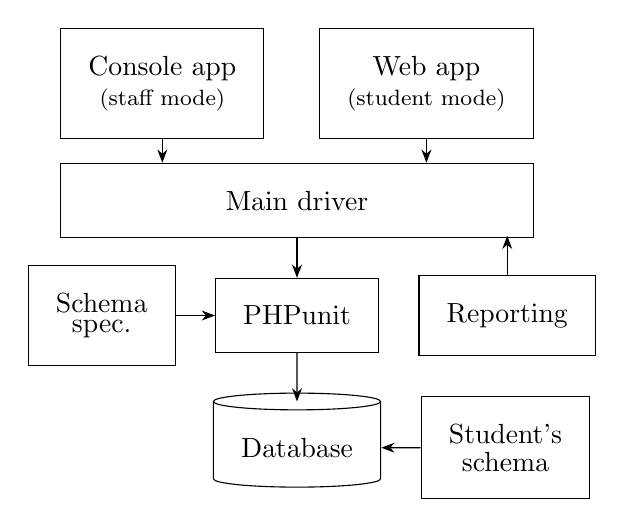
\begin{tikzpicture}[every node/.style={draw, minimum height=7.5mm, inner sep=1em}]
        \node (console) {\shortstack{Console app \\ \footnotesize(staff mode)}};
        \coordinate[below=3mm of console.south] (console port);
        
        \node[anchor=north west, minimum width=6cm] (driver) at ($(console.south west) - (0,3mm)$) {Main driver};
        
        \node[anchor=south east] (web) at ($(driver.north east) + (0,3mm)$) {\shortstack{Web app \\ \footnotesize(student mode)}};
        \coordinate[below=3mm of web.south] (web port);
        
        \node[below=5mm of driver] (phpunit) {PHPunit};
        
        \node[left=5mm of phpunit] (spec) {\shortstack{Schema \\ spec.}};
        
        \node[right=5mm of phpunit] (reporting) {Reporting};
        \coordinate[above=5mm of reporting.north] (reporting port);
        
        \node[cylinder, shape border rotate=90, below=5mm of phpunit, aspect=0.1] (database) {Database};
        
        \path (database.before top) -- (database.after top) coordinate[midway] (dbtop);
        
        \node[right=5mm of database] (schema) {\shortstack{Student's \\ schema}};
        
        \graph { [edges={draw, arrows={-{Stealth}}}]
            {(console), (web), (reporting)} -> {(console port), (web port), (reporting port)},
            {(driver), (spec)} -> (phpunit),
            (phpunit) -> (dbtop),
            (schema) -> (database),
        };
    \end{tikzpicture}
    \caption{System architecture.}
    \label{fig-architecture}
\end{figure}

There are surprisingly few frameworks for performing unit tests that interact with a database, probably due to the complexities involved. In conventional application unit testing it is relatively simple to create mocked interfaces for testing purposes. With a database, however, we need to create tables, populate them with appropriate test data, verify the state of the database after each test has run, and clean up the database for each new test \cite{Bergmann.S-2017a-PHPUnit}. Cleaning up is particularly crucial, as the order of tests is not guaranteed to be deterministic. Tests that change the state of the database may therefore affect the results of later tests in unpredictable ways.

We are only aware of four unit testing frameworks that provide specific support for database unit tests: DbUnit for Java,\footnote{http://dbunit.sourceforge.net/} DbUnit.NET,\footnote{http://dbunit-net.sourceforge.net/} Test::DBUnit for Perl,\footnote{http://search.cpan.org/~adrianwit/Test-DBUnit-0.20/lib/Test/DBUnit.pm} and PHPUnit.\footnote{https://phpunit.de/} We chose to implement the system in PHP, as it enabled us to quickly prototype the system and simplified development of the student-facing web application.

The system can be easily adapted for use with any DBMS supported by PHP's PDO extension.


\subsection{The main driver}

The core of the system is the \emph{main driver} component shown in \cref{fig-architecture}. This can execute in either \emph{student mode}, which runs only a subset of the available tests, or in \emph{staff mode}, which runs all available tests. The mode is determined by the client application, as shown in \ref{fig-architecture}. Currently student mode is accessed through a web application, while staff mode is accessed through a console application.

The main driver uses the \textbf{reporting} module to generate test output in either HTML (student mode) or plain text (staff mode).


\subsection{Encoding the assignment specification}

The assignment specification is encoded as a collection of subclasses of the PHPUnit TestCase class. Each class specifies the properties of a particular database table. \Cref{fig-test-class} shows a fragment of the class corresponding to the \textsf{Product} table from \cref{fig-ERD}. The methods of this class return various properties of the table as follows:

\begin{description}
    \item[\texttt{getTableName()}] returns the expected name of the table.
    \item[\texttt{getColumnList()}] returns an array of column specifications, keyed by expected column name. Each column specification includes a generic data type (text, number, date, or binary), a list of corresponding SQL data types (e.g., \texttt{varchar}, \texttt{decimal}), whether the column permits nulls, and a known legal value for general testing. Where applicable, it may also include minimum and maximum column lengths, and the number of decimal places. Underflow and overflow values, and lists of known legal and illegal values can be used for test the boundary conditions of integrity constraints.
    \item[\texttt{getPKColumnList()}] returns the list of columns that comprise the primary key of the table.
    \item[\texttt{getFKColumnList()}] returns an array of foreign key specifications (where applicable), keyed by the name of the referenced table. Each specification contains the list of columns that comprise that foreign key. 
\end{description}

% Teacher has complete control over what tests are run, so quite feasible to add custom properties beyond those already specified.

\begin{table}
    \footnotesize
%     \hrule
    \begin{verbatim}
public function getTableName() {
  return 'PRODUCT';
}

public function getColumnList() {
  return array(
    'PRODUCT_CODE' => array(
      'generic_type' => 'NUMBER',
      'sql_type' => array('NUMBER', 'INTEGER'),
      'min_length' => 8, 'max_length' => 8, 'decimals' => 0,
      'test_value' => 87654321, 'nullable' => false),
    'DESCRIPTION' => array( ... ),
    'STOCK_COUNT' => array(
      'generic_type' => 'NUMBER',
      'sql_type' => array('NUMBER', 'INTEGER'),
      'min_length' => 5, 'max_length' => 6, 'decimals' => 0,
      'underflow' => -1, 'overflow' => 100000,
      'legal_values' => array(0, 99999), 'test_value' => 456,
      'nullable' => false),
    'RESTOCK_LEVEL' => array( ... ),
    'MINIMUM_LEVEL' => array( ... ),
    'LIST_PRICE' => array(
      'generic_type' => 'NUMBER',
      'sql_type' => array('NUMBER', 'INTEGER'),
      'min_length' => 7, 'max_length' => 8, 'decimals' => 2,
      'underflow' => -0.01, 'overflow' => 100000.00,
      'legal_values' => array(0, 99999.99), 'test_value' => 123.99,
      'nullable' =>  false),
    'ASSEMBLY_MANUAL' => array(
      'generic_type' => 'BINARY',
      'sql_type' => array('BLOB'),
      'test_value'    =>  "NULL",
      'nullable' => true),
    'ASSEMBLY_PROGRAM' => array( ... )
  );
}

public function getPKColumnList() {
  return array( 'PRODUCT_CODE' );
}

public function getFKColumnList() {
  return array();   // no FKs in this table
}   \end{verbatim}
%     \hrule
    \caption{Fragment of the \textsf{Product} table specification.}
    \label{fig-test-class}
\end{table}


\subsection{Specifying tests}

Each table specification also requires two separate sets of tests to run on the database. The first set of tests verifies the structural elements of the table (columns, data types, etc.), thus verifying the submission meets the minimum requirement. An empty data fixture is required to support this set of tests.

The second set of tests verifies the behavioural elements of the table, i.e., it's constraints. The only integrity constraints that are tested directly are nullability, and primary and foreign keys. The behaviour of all other constraints is tested by specifying appropriate lists of legal and illegal values, which is consistent with standard unit testing techniques. A known-valid data fixture is required to support this set of tests.


% ANSI terminal colours for Terminal.app; see https://en.wikipedia.org/wiki/ANSI_escape_code#Colors
% grey 203, 204, 205
% green 37 188 36
% red 194, 54, 33
\definecolor{test grey}{rgb}{0.796,0.800,0.804}
\definecolor{test green}{rgb}{0.145,0.737,0.141}
\definecolor{test red}{rgb}{0.761,0.212,0.129}

\tcbset{boxsep=0pt, boxrule=0pt, arc=0pt, left=0pt, right=0pt, top=0.5pt, bottom=0.5pt}


\subsection{Student mode (web application)}

After creating tables under their personal database acccount, a student enters their database login credentials into a web form, which enables the main driver to access their schema directly. Only the structural tests are run, and their output appears in the web browser. \Cref{fig-student-output} shows an example of the kind of output produced in student mode.

\begin{figure}
    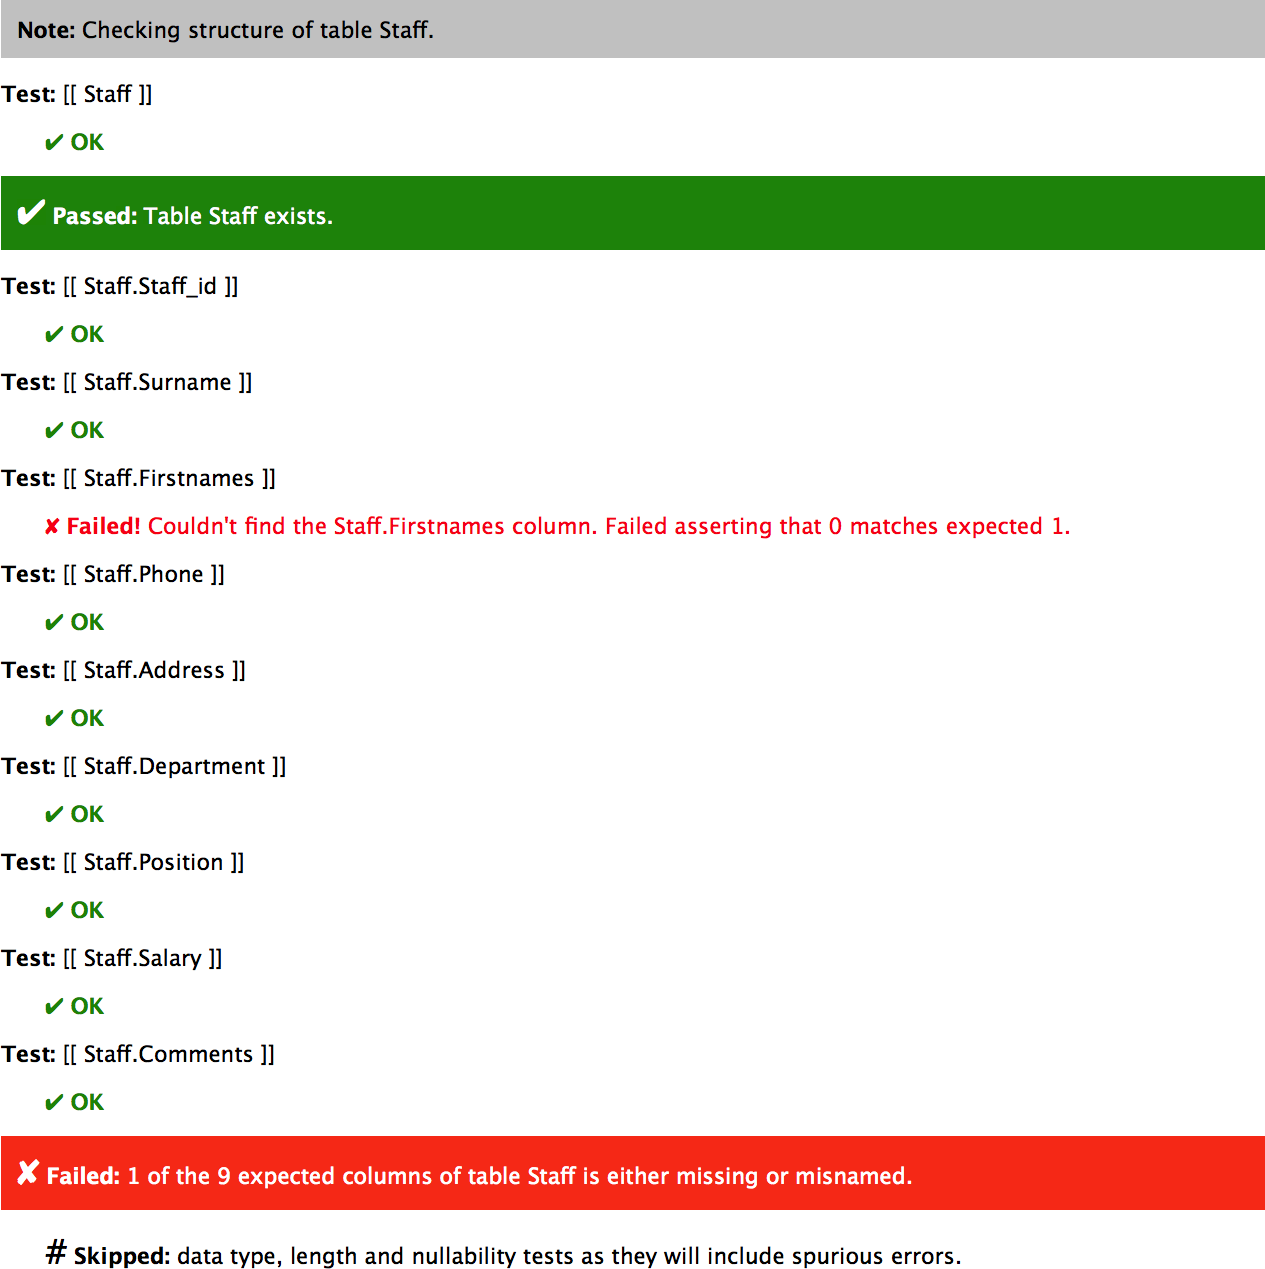
\includegraphics[width=0.95\columnwidth,keepaspectratio]{images/web_output.png}
    \caption{Example of student mode output (web app). Grey indicates informative notes, green indicates passed tests, and red indicates failed tests.}
    \label{fig-student-output}
\end{figure}


\subsection{Staff mode (console application)}

In staff mode, the database login credentials of the teacher doing the grading are specified in the console application's configuration file. The teacher loads the student's submitted SQL code into the DBMS, and then runs the console application (assuming, of course, that there are no syntax errors in the code). The main driver connects to the teacher's schema, and runs all available tests. The output of the tests appears in the terminal window. \Cref{fig-staff-output} shows an example of the kind of output produced in staff mode.

\newlength{\dothskip}
\setlength{\dothskip}{0.72cm}
\newlength{\dotvskip}
\setlength{\dotvskip}{-1.25ex}
\newlength{\codeskip}
\setlength{\codeskip}{-0.5ex}

\begin{figure}
    \ttfamily\scriptsize
    \begin{tabbing}
        0123\=\kill
        \tcbox[colback=test grey]{NOTE: Checking structure of table Product.} \\[\codeskip]
        TEST: [[ Product ]]  \\
        \>  \textcolor{test green}{+ OK} \\
        \tcbox[colback=test green]{+++ PASSED: Table Product exists.} \\[\codeskip]
        TEST: [[ Product.Product\_code ]]  \\
        \>  \textcolor{test green}{+ OK} \\[\dotvskip]
        \hspace*{\dothskip}\vdots \\
        \tcbox[colback=test green]{+++ PASSED: Table Product contains all the expected columns.} \\[\codeskip]
        TEST: [[ Product.Product\_code: data type is NUMBER | INTEGER ]]  \\
        \>  \textcolor{test green}{+ OK} \\[\dotvskip]
        \hspace*{\dothskip}\vdots \\
        \tcbox[colback=test green]{+++ PASSED: All columns of table Product have data types compatible with the}\\[\codeskip]
        \tcbox[colback=test green]{specification.} \\[\codeskip]
        TEST: [[ Product.Product\_code precision and scale = 8 (with scale 0) ]]  \\
        \>  \textcolor{test green}{+ OK} \\[\dotvskip]
        \hspace*{\dothskip}\vdots \\
        \tcbox[colback=test green]{+++ PASSED: All columns of table Product have lengths compatible with the} \\[\codeskip]
        \tcbox[colback=test green]{specification.} \\[\codeskip]
        TEST: [[ Product PK ]]  \\
        \>  \textcolor{test green}{+ OK} \\
        \tcbox[colback=test green]{+++ PASSED: Primary key of table Product exists.} \\[\codeskip]
        TEST: [[ Product PK: Product\_code ]]  \\
        \>  \textcolor{test green}{+ OK} \\
        \tcbox[colback=test green]{+++ PASSED: Primary key of table Product includes (only) the expected} \\[\codeskip]
        \tcbox[colback=test green]{columns.} \\[\dotvskip]
        \hspace*{\dothskip}\vdots \\
        \tcbox[colback=test grey]{NOTE: Testing constraints of table Product.} \\[\codeskip]
        TEST: [[ Product.Stock\_count accepts ``0'' ]]  \\
        \>  \textcolor{test green}{+ OK} \\
        TEST: [[ Product.Stock\_count accepts ``99999'' ]]  \\
        \>  \textcolor{test green}{+ OK} \\
        TEST: [[ Product.Restock\_level accepts ``0'' ]]  \\
        \>  \textcolor{test red}{- FAILED! Column Product.Restock\_level won't accept legal value 0.} \\
        \textcolor{test red}{Failed asserting that false is true.} \\
        TEST: [[ Product.Restock\_level accepts ``99999'' ]]  \\
        \>  \textcolor{test green}{+ OK} \\
        TEST: [[ Product.Minimum\_level accepts ``0'' ]]  \\
        \>  \textcolor{test red}{- FAILED! Column Product.Minimum\_level won't accept legal value 0.} \\
        \textcolor{test red}{Failed asserting that false is true.} \\
        TEST: [[ Product.Minimum\_level accepts ``653'' ]]  \\
        \>  \textcolor{test green}{+ OK} \\[\dotvskip]
        \hspace*{\dothskip}\vdots \\
        \tcbox[colback=test red, coltext=test grey]{--- FAILED: 2 of 8 legal values tested were rejected by a CHECK constraint.}
    \end{tabbing}
    \vskip-1ex
    \caption{Example of staff mode output (console app).}
    \label{fig-staff-output}
\end{figure}


\section{Evaluation}
\label{sec-evaluation}

Unfortunately, the system was implemented more as a practical solution to a perceived problem, without consideration for any formal evaluation. We therefore did not carry out any formal evaluations with students.

However, we did have detailed records of student performance on the relevant assignment, which was of the nature discussed in \cref{sec-motivation}. The assignment was counted for 15\% of the overall grade in 2009 and 2010, and 10\% in the years following.  We extracted data for the period 2009--2016, which encompassed several different permutations of scenario and system components used, as summarised in \cref{tab-data}.

\begin{table}
    \begin{tabular}{rrrll}
        \toprule
                        &   \textbf{Cohort} &   \textbf{Mean}   &                       &   \textbf{Components}  \\
        \textbf{Year}   &   \textbf{size}   &   \textbf{(\%)}   &   \textbf{Scenario}   &   \textbf{used}\\
        \midrule
        2009    &   46  &   77.5    &   ``postgrad''        &   --  \\
        2010    &   68  &   73.4    &   ``student records'' &   --  \\
        2011    &   64  &   71.8    &   ``used cars''       &   --  \\
        \midrule
        2012    &   75  &   69.2    &   ``BDL''             &   staff   \\
        2013    &   77  &   84.3    &   ``student records'' &   student/staff \\
        \midrule
        2014    &   49  &   77.6    &   ``used cars''       &   student/staff \\
        2015    &   71  &   69.2    &   ``used cars''       &   --  \\
        2016    &   75  &   71.0    &   ``BDL''             &   staff   \\
        \bottomrule
    \end{tabular}
    \caption{Characteristics of student grade data.}
    \label{tab-data}
\end{table}

The two horizontal rules in \cref{tab-data} indicate two major transitions during this period. The first marks a significant reorgansation of the paper's curriculum (and a switch from first to second semester\footnote{Semesters at the University of Otago run from March to June and July to October.}) in 2012, the year the prototype of our system was developed. The second marks a shift from second semester back to first semester in 2014. Note that the system was not used at all in 2015 due to different staff teaching the paper. The student component was not used in 2016 due to technical issues. This natural experiment provides us with some interesting points for comparison.

Grades for the assignment drifted slowly downwards from 2009 to 2012. This changed dramatically in 2013, however, the year that the student component of our system was introduced. The grades are not normally distributed (they typically have negative skew), so we performed a Wilcoxon signed-rank test to check whether this difference in mean was statistically significant. The difference proved to be highly significant (\(p \approx 10^{-9}\)). The 2013 grades were also significantly higher than those of 2010 (\(p \approx 0.0002\)) and 2011 (\(p \approx 10^{-6}\)), but not significantly higher than 2009. The mean dropped significantly again in 2014, the second year that the system was used (\(p \approx 0.0012\)), and again in 2015 (\(p \approx 0.0005\)), when the system was not used at all. There was no significant change from 2015 to 2016.

More interesting, if we compare the performance between the years that the student component was available (2013--2014, mean 81.7\%) and the years it was not (2009--2012, 2015, 2016, mean 71.6\%), there is again a highly statistically significant difference in the mean (\(p \approx 10^{-8}\)). This suggests that the student component may have had a positive effect on students' ability to complete the assignment more effectively.

\subsection{Potential confounding factors}

2013 was also the first year that the assignment specification was enforced as being ``frozen''. It could be argued that this improved grades due to students having less flexibility, and thus less opportunity for misinterpretation, than in previous years. However, the assignment specification was also ``frozen'' from 2014--2016, and there is notable variation in the grades achieved over this period. It therefore seems unlikely that this is a factor in improved assignment performance.

Results for first semester offerings of the paper (2009--2011 and 2014--2016, mean 72.9\%) were significantly lower (\(p \approx 0.014\)) than those for second semester offerings (2012--2013, mean 76.9\%). However, since the paper was only offered twice in the second semester over this period, this seems unlikely to be cause the difference. The higher results are more likely due to the large jump in grades in 2013, which had the highest grades over the entire period.

% Anecdotal evidence from students?

% known issues:
% There's currently no control over the messages generated by PHPUnit assertions. You can put a meaningful message up front, but PHPUnit will still always generate something like ``Failed asserting that 0 matches expected 1.'' This can be particularly misleading when you, e.g., don't specify a precision for a numeric column, and the DBMS uses the default precision (e.g., Oracle's NUMBER defaults to 38 significant digits).
% A partial schema causes a large number of errors, as tables don't exist. This could be alleviated by more careful exception handling?
% Students in the first iteration tended to misuse the web application as a ``schema compiler'', fixing only one issue before re-submitting, rather than attempting to fix as many of the reported problems as possible. The system wasn't written to handle concurrent requests (as it wasn't expected that the request rate would be that high), leading to waits and timeouts. A workaround was to enable logging, and warn students who were abusing the system.

Another possibility is that grade performance is related to the complexity of the scenario. We computed a few different database complexity metrics \cite{Jamil.B-2010a-SMARtS,Piattini.M-2001a-Table,Pavlic.M-2008a-Database,Calero.C-2001a-Database,Sinha.B-2014a-Estimation} for each of the four scenarios used. According to the metrics, the ``BDL'', ``used cars'', and ``student records'' scenarios all had similar levels of complexity, while the ``postgrad'' scenario had a complexity score about \(\frac{2}{3}\) that of the other three. It therefore seems unlikely that scenario complexity is a factor in the difference in grades. It's also interesting to note that the ``used cars'' scenario was used in both 2014 and 2015, and that the 2015 results are significantly lower than those for 2014. The only obvious difference here is that our system was not used at all in 2015.

\section{Conclusions \& future work}
\label{sec-conclusion}


\bibliographystyle{ACM-Reference-Format}
\bibliography{Koli_2017_Stanger}

\end{document}
